
\documentclass[12pt, letterpaper]{article}
\usepackage{fontspec}
\usepackage{listings}
\usepackage{booktabs,caption}
\usepackage[flushleft]{threeparttable}
\usepackage[margin=2.5cm]{geometry}
\usepackage{amsmath}
\usepackage{graphicx}
\usepackage{booktabs}
\usepackage{longtable}
\usepackage[colorlinks=true, allcolors=blue]{hyperref}
\usepackage{amssymb, amsfonts, amsmath}
\usepackage{bm}
\usepackage{setspace}               % line spacing
    \onehalfspacing
\usepackage{adjustbox}              % resizing
\usepackage{caption}                % to reset the cations etc 
\usepackage{rotating}               % for the sidewaystable
    \numberwithin{table}{section}   % reset the Table numbering for each section
\usepackage{booktabs}               % neatly formatting lines
\usepackage{dcolumn}                % aligning decimals
    \newcolumntype{d}[1]{D{.}{.}{#1}}
\usepackage{natbib}                 % bibliography
    \bibliographystyle{plainnat}

\newcommand{\sym}[1]{\rlap{#1}} % for the stars
\setmainfont{Times New Roman}
\title{\textbf{Labor Share of Income:\\ An Empirical Analysis of the Last 15 Years}}
\author{Francisco Alvarez, Leonardo Endrizzi, Samuli Salonen}
\date{\today}

\renewcommand{\baselinestretch}{1.5}
\begin{document}

\maketitle
%%abstract
\begin{abstract}
	This paper aims to figure out the dynamics of the labor share of income in the last fifteen years. In the first part of the paper, we look at the dynamics in the world share of income, then we analyze this ratio by dividing countries by their level of income and in the end, we see if there are some countries with some particularly interesting dynamics. Given that premises, in the second part, we address our interest in the reasons of why we can have different dynamics in the labor share of income. Moreover we are interested in understanding if using trade openness, capital intensity, and total factor productivity which normally explain the dynamics in the long run can also explain it in the short run.
\end{abstract}
%TC:ignore
% Keywords command
\providecommand{\keywords}[1]
{
  \small	
  \textbf{\textit{Keywords---}} #1
}
\keywords{Labor Share, Econometrics, Panel Data}

\section{Introduction}\label{sec_1}
One common debate among economists in the last years is the dynamics of the labor share of income. This topic has become relevant for two main facts: its strict relation with income inequality, and its relevance in the standard macroeconomic theory. Since Kaldor (1957) the standard assumption has been that the ratio between workers' compensation and economic output is constant over time. But in a more recent analysis, (see Piketty (2014)) it is observed that in fact, the global labor share of income is decreasing. We will analyze the labor share of income for the last fifteen years, to understand if changes happen in the short run, or if we can consider Kaldor's assumption true in the short run and Piketty's analysis in the long run. In the first section of this paper, we analyze the theoretical framework in which we base our analysis on, in the second section we look at the data and visualize what are the dynamics of the labor share of income for the world in general, for countries aggregated by different levels of income, for countries divided by region and for some specific countries due to their outstanding dynamics. In the third section, we develop the analysis to explain why these changes happen, using three drivers: trade openness which takes into account the level of international trade between one country and the rest of the world, the capital intensity which represents the amount of capital per workers, and the total factor productivity which can be a proxy of the technological level of a country. In the end, we present our results and our conclusions.

\section{Literature Review}\label{sec_2}
According to Charpe, Bridji and McAdam (2020), there has been an increased interest in the study of the labor share of income, and it has been studied since the major classical economists like Smith, Ricardo, and Marx. There is a difference when studying this topic from a short-run or a long-run perspective, as results vary. There is literature with empirical support, like the study from the European Union (2007) in which they show that there is a negative movement between the labor share of income and growth.

As mentioned before, the debate on whether or not the labor share of income remains constant over time is widely studied. Rodriguez and Jayadev (2013) show in their study, using two different panel data sets starting from 1980 how the labor share of income has decreased globally. The determinants of the labor share of income are greatly relevant for the understanding of the dynamics of the LSOI; Bentolila and Saint-Paul (2003) show how it is related to the capital-output ratio. In their study, they show a panel of 12 OECD countries from 1970 to 1990, and on average, the labor share of income decreased by -1.1 percent for these countries. 

The econometric models used in this topic vary, but using panel data with fixed effects is identified in several of the papers that were cited. Elsby, Hobijn, and Şahin (2013) show that for a country-level study of 25 years in the United States of America, the dynamics have been different for each sector, but the decline that they find has been mainly dominated by trade and manufacturing sectors. The main variables that they use in their study are the labor share,  capital-output ratio, real price of oil, total factor productivity, employment growth rate, and labor conflict rate. It is interesting in how they take into account that for this period, oil was a really important factor for the US economy, so there are several ways in which we can look at how the LSOI is studied to find its determinants.

Hogrefe, Doan and Wan (2017) is a relevant study for this paper, since they developed estimations for their model accounting for country fixed effects. We follow their methodology on the calculation for capital intensity; their model also accounts for outward foreign direct investment and inward foreign direct investment, but they end up finding that those variables are not significant in the construction of their model. However, there are studies that show that adding the foreign direct investment effect does have an impact. Decreuse and Maarek (2015), showed how an inward foreign direct investment depressed the labor share. An interesting thing that is mentioned, is that when there are variables that are correlated with GDP per capita, they could also be correlated with the labor share.

What we develop in the next sections is based on what previous studies have found, taking into account what variables have been used classically and the main methods that are used to study countries over a different period of time, and focusing mainly on the different levels of LSOI for the different income groups. Moreover, we would like to see if the decreasing of the labor share of income is a long run trend or if it could be seen also in the short and medium period. In the end, we want to understand if the variables that are relevant for long period are also relevant in the short and medium run.
%, since it shows the various levels of capital and labor for these groups, this being our main contribution for the literature regarding this field.

%we need to connect what previous studies died and connect them to what we are doing 


\section{Theoretical Framework}\label{sec_3}
The labor share of income ($LSOI$) is defined as the total labor compensation over the nominal output. It is needed to do a lot of assumptions, if we want to show it briefly in a mathematical way. These include having only one representative firm, one product given by $F(K(t),L(t))$, one price $P(t)$ and one level of wages $w(t)$. As a consequence we have
\begin{equation*}
    LSOI(t) = \frac{w(t)L(t)}{P(t)F(K(t),L(t)}
\end{equation*}
Here it is possible to see the principal drivers of the changes: 
\begin{enumerate}
    \item Wages - an increase in wages drives an increase in the LSOI, firstly because wages are on the numerator of the fraction but also an increase in wages has a positive effect on the labor supply but a negative effect on production, because labor costs more;
    \item Number of workers - an increase in the number of workers leads to an increase in the labor share of income if we consider its effect alone. Notably, however, an increase in the number of workers means also a decrease in wages and an increase in production;
    \item Prices are at the denominator of the ratio, but if instead we consider the wages as real wages, we can give less weight to  this variable; however, taken as constant the other variable, an increase in prices leads to a decrease in the LSOI. But then again if we consider the secondary effects wages are normally indicized to prices they will increase at the same rate;
    \item Production: an increase in production leads to a decrease in LSOI if we consider as constant the other variables, but in fact an increase in production if led by technological progress influences also prices, the number of workers, and wages.
\end{enumerate}
To complete the basic framework, it is assumed that the production function is of the form $F(K(t),L(t)) = K(t)^\alpha L(t)^{1-\alpha}$ (i.e. we have a Cobb-Douglas production function) we can calculate the LSOI as:
\begin{equation*}
    LSOI(t) = \frac{w(t)L(t)}{F(K(t),L(t)} = \frac{(1-\alpha)K^{\alpha} L^{1-\alpha}}{K(t)^{\alpha} L(t)^{1-\alpha}} = 1 - \alpha
\end{equation*}
and as a consequence, we can define the capital share of income (CSOI) as $\alpha$. 
In this case, given the numerous assumptions behind the Cobb-Douglas function\footnote{It is obvious that this function is too easy to represent a modern economy, but it allows us to give an idea of the reasoning behind it.}, we see that the labor share of income is constant. To understand well the dynamics of the labor share of income, we need to  develop this framework and to modify the production function in order to make it more realistic and to find what  can influence $\alpha$. It is clear that what is missing at the moment is some technological progress which is one of the most important driver of an economy since the industrial revolution. Following the paper from Bentolila S. \& Saint-Paul G., if we assume that there is a labor-augmenting technical progress, $B$, such that $Y = F(K(t),B(t)L(t)$ then it is possible to prove that there exists a unique function $g$ such that:
\begin{equation*}
    LSOI(t) = g(k(t))
\end{equation*}
where $k(t)$ represent the capital-output ratio $k(t) = K(t)/L(t)$.
It's explicit form is:
\begin{equation*}
    LSOI = kh(k)f'(h(k))
\end{equation*}
where we have erased the dependence on time $t$ only for simplicity of notation and we have transformed the variables in per capital terms and as a consequence $k=1/f(l)$ where $l = BL/K$, $f = F(1,BL/K))$ and $h(k) = f^{-1}(1/k)= l$. 
It is important here to note that the response of the LSOI to the capital-output ratio is strictly related to the elasticity of substitution between capital and labor.
But if we include capital-augmenting technical progress, so that the production function is of the form $F(AK,BL)$, this relation between labor share of income and capital-output ratio is no longer stable, and is represented by:
\begin{equation*}
    SLOI = Akf(Ak)f'(g(Ak))
\end{equation*}
As a consequence, changes in A, shift the labor share of income.
The other fact we want introduce in our theoretical framework is the difference between the marginal product of labor and the real wage justified by the product market power\footnote{See Bentolila S. \& Saint-Paul G.(2003) for more details.}.
Assuming imperfect competition, it is well known from microeconomic theory that there is a markup $\mu$ of prices on marginal costs. As a consequence, deriving the production function by labor we obtain:
\begin{equation*}
    \frac{\partial F}{\partial L} = Bf'(l) = (1+\mu) \frac{w}{p}
\end{equation*}
and using it in the calculus of the labor share of income:
\begin{equation*}
    LSOI = (1+\mu)^{-1}\frac{lf'(l)}{f(l)}
\end{equation*}
or compactly $LSOI = (1+\mu)^{-1}g(k)$. This means that if competition increases, the mark-up will decrease and labor share of income will increase, and vice-versa.  We will use this framework to develop the econometrics model in section 5.

%Maybe this section we should add something more!!


\section{Data Explanation and Visualization}\label{sec_4}

To analyze the dynamics of the labor share of income we use the data from the International Labor Organization (ILO)\footnote{https://ilostat.ilo.org/data/} and the Penn World Table (PWT)\footnote{https://www.rug.nl/ggdc/productivity/pwt/?lang=en}. Our data set is represented by panel data for $153$ countries and $16$ years.

It is important to have a clear visualization of the variable of interest of this paper\footnote{There are different ways on how the LSOI is calculated, see Gutiérrez, Germán, and Piton, (2020)}.
In figure 1. we can see the dynamics of the labor share of income at the aggregate level. At a first glance, it is possible to note that the difference between 2004 and 2019 is not large, but there is an important pick in correspondence with the Great Recession of 2009 that could have compromised the decreasing trend started in the years before.

Aggregating the data globally is not very significant:
The first attempt to understand better the dynamics of the labor share of income is to divide the countries into four different levels of income (high income, upper middle income, lower middle income, and low income\footnote{This division is taken from the World Bank database, with no further analysis.}). What becomes clear using this classification (see Figure 3.) is that more developed countries have a higher LSOI\footnote{Even though it is not the purpose of this paper, it is possible to understand why poor countries have less LSOI: controlling for GDP, the level of wages is lower with respect to rich countries}, but we cannot infer a lot about the dynamics. As we have seen for the world, the crisis of 2009 has had a positive impact on all the countries, independently from their income (see in the next section the inclusion of a dummy variable for the crisis).

Another possible strategy to analyze the labor share of income is to divide countries by region\footnote{Also these division is taken from the World Bank database.}. As before, belonging to a different region  implies a different level of LSOI. This is not surprising, because the countries in North America and Europe and Central Asia are the richest and as seen before, they have the largest share. Meanwhile, countries in the Middle East and North Africa are the poorest and have the lowest share. Nonetheless, it is very difficult to see a substantial variation in the LSOI in the last fifteen years.  

To complete this section we have a look at all the countries' dynamics of the share of income, as we can see in Figure 4., Figure 5., Figure 6., Figure 7. and Figure 8. the majority of the countries do not have a significant change in the variable of interest, therefore by aggregating the data we do not lose a lot of information about the real movement of the LSOI. However, observing carefully the data we can note two anomalies: the first one is represented by Argentina, Belarus, Azerbaijan, Bulgaria, Ecuador, and Georgia for which the Labor Share of Income increased by 10 percentage points circa during the last fifteen years. This is particularly relevant if it is noted that all these countries belong to the upper middle-income category, and that an increase in LSOI is not predicted by the theory.

The other interesting oddities are the United Arab Emirates and Qatar: Even though both United Arab Emirates and Qatar belong to high-income countries, they have a very low labor share of income $20\%$ in 2004, and $35\%$ and $25\%$ in 2019, respectively, when instead the mean for high-income countries is $52.5\%$. This is a consequence of the fact that in these countries the GDP is really high, but the distribution of it is really unequal and salaries are very low for the majority of the workers.

\section{Econometric Model}\label{sec_5}
In the previous section, we visualized the data and we noticed a common path: the labor share of income doesn't change much in the short run. This could be a problem for the significance of our econometric model because if the independent variable has a very low variance, it is difficult to obtain a high value for the $R^2$. On the other hand, this could be important for the purpose of this paper that analyzes the dynamics of the LSOI in the short run. Other important considerations that we want to take into account are the role of different levels of income of the countries and the effect of the crisis\footnote{We don't analyze LSOI using the different regions because to control for regions is not enough to obtain good results: for example, it is well known that there is a correlation between poor countries and where they are located, so we should also control for income in that case, and in some sense we return to the income group classification.}.

To have a more precise analysis of the data about the LSOI it is possible to see Table 5.1: as we have seen also graphically before, the mean for the World during the fifteen years is $47,18\%$ but with a large standard deviation of $9.5$. More interesting are the statistics between the countries and the within a single country. In fact, we see that the variability between the countries is much more important and this suggests that the labor LSOI doesn't change much during the fifteen years of interest. 

%here we add the table : xtsum of lsoi!!
\begin{table*}[htbp!]
\small
\caption{\textbf{\textit{Summary Statistics for LSOI}}} \label{tab:sumlsoi}
    \begin{center}
            {
    \def\sym#1{\ifmmode^{#1}\else\(^{#1}\)\fi}
    \begin{tabular}{l*{1}{ccccccc}}
    \hline\hline
    Variable &         & Mean     & SD & Min      & Max      & Observations \\
    \hline
    lsoi     & overall & 47.17955 & 9.498049  & 14.94    & 76.48    & N =    2448  \\
             & between &          & 9.194935  & 19.85125 & 67.86375 & n =     153  \\
             & within  &          & 2.486842  & 31.98892 & 62.09892 & T =      16 
    \end{tabular}
    }
    \end{center} 
\centering\footnotesize Source: Own elaboration with data from ILOSTAT
\end{table*}

Moreover following the literature, to understand the labor share of income dynamics it is common to use globalization  and technological change.
Globalization is a very complex concept, so we will focus only on international trade:  it's an important factor for competitiveness  and "exerts downward pressure on the labor share" (Hogrefe, Kappler 2012). We will use as a proxy of the relationship between a country and the rest of the world the \textbf{trade openness} ($openness$), defined as the difference between imports over GDP and exports over GDP. 

The other fundamental driver of an economy in general and a factor that can help to understand the labor share of income changes is technology. The measure of technology, and as a consequence technological progress, is another poser for economists. The most common in this framework (see Hogrefe, Kappler(2012) and Ha Thi Than Doan, Guanghua Wan (2017)) is to use \textbf{total factor productivity}, TFP ($ctfp$). This is justified by the fact that  TFP affects the labor share of income: if the technological progress is capital-augmenting, then this means that an increase in technology will drive a decrease in labor, and as a consequence in the LSOI, and the other way around if the technology is labor-augmenting. In our data, we have a lot of missing values for this variable, and by analyzing them it is possible to observe that normally it happens for countries in the low income or lower-medium income categories. As a consequence, we have decided to use a dummy variable ($dftp$) which compares the TFP of a single country with the mean for the world every year. If it is below the mean, it will be $0$, and if not, it will be $1$. For the countries for which we don't have the data, the value will be 0.

We want to include also \textbf{capital intensity} as a control variable, normally indicated as $k$, and in the regression as $capitalint$, because it is important to take into account the factor endowment. The relation to the labor share of income is given by the elasticity of substitution between labor and capital: if they are complementary (substitutes), then an increase in the $k$ leads to a decrease (increase) in the labor share. We will use the logarithm of $capitalint$, which we will call $lcapitalint$ for interpretation reason. 

%here the summary for all the variable!

\begin{table*}[htbp!]
\small
\caption{\textbf{\textit{Summary Statistics for Explanatory Variables}}} \label{tab:sum}
    \begin{center}
        {
\def\sym#1{\ifmmode^{#1}\else\(^{#1}\)\fi}
\begin{tabular}{l*{1}{cccc}}
\hline\hline
            &        Mean&          SD&         Min&         Max\\
\hline
lsoi        &       47.18&        9.50&       14.94&       76.48\\
dtfp        &        0.35&        0.48&        0.00&        1.00\\
openess     &       -0.06&        0.17&       -0.85&        0.76\\
lcapitalint &       11.44&        1.34&        8.03&       13.80\\
\hline\hline
\end{tabular}
}

    \end{center} 
\centering\footnotesize Source: Own elaboration with data from ILOSTAT and Penn World Table
\end{table*}

In Table 5.2, it is possible to see a summary of all the explanatory variables: we have commented before the LSOI, so we will briefly have a look at the others. The $dtfp$ has a mean of $0.35$, summarizing the fact that more countries have a total factor productivity below the mean. The negative mean of the $openness$ means that countries have normally a trade deficit of $6\%$ of the GDP, but with high standard deviation, so it differs a lot from country to country. Lastly, $lcapitalint$ has a mean of $11.44$ which doesn't have a lot of significance because it's the logarithm of the capital intensity; the standard deviation in this case is not large.\\

The basic model that we want to analyze is given by:
\begin{equation*}
    lsoi_{i,t} = \beta_0 + \beta_1 openness_{i,t} +\beta_2 dftp_{i,t} + \beta_3 capitalint_{i,t} + \mu_{i,t}
\end{equation*}

%here the table with the simple regression!!!!

This model is for sure incomplete. The first important change we want to do is controlling for the \textbf{financial crisis of 2008}. As we have seen in the previous section, the financial crisis affected all the countries and at a global level could have compromised the decreasing of the LSOI. We introduce it as a dummy variable $crisis$, which assumes value of $1$ when $year = 2009$ and value of $0$ in all the other years. This could not be very clear, but due to the fact that the crisis happened in $2008$ and that the dataset is compiled only once a year, we can account for the crisis only in $2009$. As a consequence the updated model will be:
\begin{equation*}
    lsoi_{i,t} = \beta_0 + \beta_1 openness_{i,t} +\beta_2 dftp_{i,t} + \beta_3 capitalint_{i,t}  + \beta_3crisis_t + \mu_{i,t}
\end{equation*}

Moreover, remembering again what we have observed before, countries can be divided in four \textbf{different groups based on their income level}. As Lee and Kim (2009) have shown that countries with the same level income have a lot of other  characteristics in common as well as policies affect different income groups differently \footnote{We can note that one of them is also the LSOI: if we observe the standard deviation of LSOI dividing the countries by their level of income in fact we can observe that it is less than the entire word; the only exception is the high income countries, but this is a consequence of the inclusion of United Arab Emirates and Qatar in this category.}. As a consequence, we think we can use the income groups, $incg$, as a categorical variable that can be thought as a \textbf{fixed effects}. The up-to-date model is:
\begin{equation*}
    lsoi_{i,t} = \beta_0 + \beta_1 openness_{i,t} +\beta_2 dftp_{i,t} + \beta_3 capitalint_{i,t}  + \beta_3crisis_t + \beta_4incg+ \mu_{i,t}
\end{equation*}

%Discussion about Random Effect
Thinking about including \textbf{random effects}, in which unit-specific effects for all units are distributed around a common mean value, doesn't sound viable. In fact it's like assuming that the mean of labor share of income is behind every country but the values that we observe it's the consequence of an unknown distribution. 

%Discussion about Heteroschedasticity

% Discussion about Endogeneity


\section{Results}\label{Results}
In this part, we will analyze the regression tables based on the models we have developed in the previous sections.
Note that all the regressions are built using robust estimators to cope with heteroskedasticity of the data.
Looking at the first model, see Table 8.1, we can see the regression model using Pooled OLS, OLS with Random Effects, and OLS with Fixed Effects. 
In all three models, we look at the coefficients, the signs, and the magnitudes. Firstly, looking at Pooled OLS we can see that all the explanatory variables are significant but if openness has a negative sign, as expected to be as a consequence of globalization, this is not the case for the total factor productivity. This means that technology is labor-biased and this is in contrast with our intuition and it can be found on the papers written by Hogrefe et al. (2017). Also, the impact of capital intensity is positive (and significant) which means that if capital labor ratio increases also the labor share of income increases, suggesting that capital and labor are complementary. Now we want to analyze the second column of the regression, with random effects for completeness: In this case, only openness with a reduced effect with respect to pooled regression and the constant is significant. In the end, we have a look at the column for fixed effect. Here, openness is significant and has the same magnitude as for random effect, and negative sign as in the other regression. We can also note that all the other explanatory variables are not significant, so not statistically different from zero but their sign follows the intuition: technology is capital biased and labor and capital are complementary. The constant moreover grows from $16.77$ and from $46.13$ to $50.35$ in pooled OLS and random effects respectively. We should also note that the $R^2$ is not so high in the first regression, about $20\%$, but is insignificant $1\%$ in the last one. 
To conclude, the Hausman test (Table 8.2) largely supports the use of fixed effects model instead of random effects model.

The second model we analyze is the same as the previous one, but we introduce the dummy variable for representing financial crisis. On one hand, someone can argue that it could be preferable to introduce time fixed effects, because it is common in economics to control for variables that are constant across units but vary over time. On the other hand, we can clearly see in the graphs that the crisis is the major change in a lot of countries and moreover it affects them differently. As a consequence, it seems more reasonable to introduce this dummy variable. 
%RELATED TO THIS SHOULDN'T WE INTRODUCE AN INTERACTION BETWEEN THE LEVEL OF INCOME AND THE DUMMY VARIABLE FOR CRISIS??
As we can see in Table 8.3 the results don't change much adding the crisis, but it's interesting to see that this variable is not significant in the pooled OLS but it is in the Random and Fixed Effects. Its sign is positive, as expected because the crisis affects GDP and not in fact fixed capital or labor, and this is why the coefficients of the other explanatory variables remain almost the same\footnote{This argument could be misleading, but here we touch two controversial topics in economics: firstly, the financial crisis and secondly, the definition of capital.}. Also, the $R^2$ doesn't improve and the Hausman test (Table 8.4) gives the same result as before.

In Table 8.5 it is possible to see the regression models with crisis and income groups. As stated in section 5, when we estimate the coefficients with fixed effects the variable $incg$ is omitted: in fact, fixed effects substitute the category variable of income level. Except that $incg$ is significant and negative in sign because of the encoding of the variable: taken as base level the $High Income$ countries ($incg = 0$), the higher the level of $incg$ ($1,2 \text{ or } 3$) the poorer the country ($Upper\text{ }middle\text{ } income, Lower\text{ } middle\text{ } income, Low\text{ } income$). In conclusion, the most significant change is that $dftp$ in the pooled OLS becomes less significant. $R^2$ increases a little in both cases, but we don't get anything from that. Also, the Hausman test (Table 8.6) remains the same.

In the end, talking about endogeneity and omitted variables at this level of analysis doesn't make a lot of sense. For sure, our model is incomplete and needs to be fixed using other variables or different techniques, as we suggest in the conclusions.

\section{Conclusions}\label{Conclusions}
%here we summarize what we have found
The purpose of this paper is to show the dynamics of the labor share of income in the last 15 years and if the variables in the literature can explain the changes of LSOI in the long run can also explain it in the short or medium run. What we have seen is that the labor share of income hasn't changed much in the last fifteen years and that the global economic crisis could have influenced it. These two facts could have been a problem for our estimates and the low $R^2$ in all the tables that we have shown. In any case, openness and also the level of income seem to be relevant. The other variables don't change much in the analysis and for fixed effects, even if they follow the economic intuition they are not significant and could be influenced by omitted variables. It is to be noted that a lot more work on the labor share of income should be done, including for example the sector composition of the economies. However, if we take our econometric analysis as valid, our paper could suggest that using the Kaldor assumption of the constant labor share of income over time in the short and the medium run, and to develop a new model that can explain the decreasing of the ratio in the long run as, Piketty (2014) has tried to do using the rate of return on capital $r$ and the capital to income ratio $\beta$. Moreover, what economists should try to understand better is how much time changes in technology and variation of capital take to show their effects on the labor share of income.


\clearpage
%%References section

\begin{thebibliography}{100}
	%Book
	\bibitem{Kaldor} N. Kaldor (1957), \textit{A Model of Economic Growth}. The Economic Journal, vol 67, Issue 268, pp. 591-624, 1957.
	 
	%EBook
 
	%Article
    \bibitem{Charpe} Charpe, M., Bridji, S., and McAdam, P. (2020). Labor share and growth in the long run. \textit{Macroeconomic Dynamics}, 24(7), 1720-1757.
    \bibitem{EC} EC (2007). The labor income share in the European Union. \textit{Employment in Europe}, 2007, p. 235-272.
    \bibitem{Rodriguez} Rodriguez, F., and Jayadev, A. (2013). The declining labor share of income.\textit{ Journal of Globalization and Development}, 3(2), 1-18.
    \bibitem{Bentolila} Bentolila, S., and Saint-Paul, G. (2003). Explaining movements in the labor share.\textit{ Contributions in Macroeconomics}, 3(1).
    \bibitem{Elsby} Elsby, M. W., Hobijn, B., and Şahin, A. (2013). The decline of the US labor share. \textit{Brookings Papers on Economic Activity}, 2013(2), 1-63.
    \bibitem{doan} Doan, H. T. T., and Wan, G. (2017).  Globalization and the labor share in national income. \textit{Asian Development Bank Institute}. Available at SSRN: https://ssrn.com/abstract=2942647 
    \bibitem{decr} Decreuse, B., & Maarek, P. (2015).DI and the labor share in developing countries: A theory and some evidence \textit{F. Annals of Economics and Statistics/Annales d'Économie et de Statistique}, 2015, 289-319.
    \bibitem{kim} Kim, B. & Lee, K. (2009). Both Institutions and Policies Matter but Differently for Different Income Groups of Countries: Determinants of Long-Run Economic Growth Revisited. \textit{World Development}, 2009, 533-549
    \bibitem{pik} Piketty, T. (2014). Capital in the Twenty-First Century, \textit{Harvard University Press}, Translated by Arthur Goldhammer, Available at: http://www.jstor.org/stable/j.ctt6wpqbc
\end{thebibliography}
\clearpage
\section{Graphs and Tables}\label{Graphs}

\begin{figure}[htp!]
    \centering
    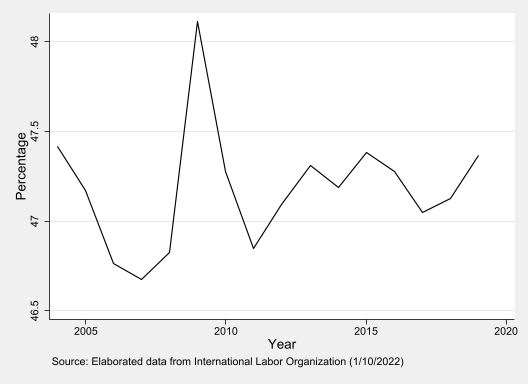
\includegraphics[width=11.5cm]{World.jpg}
    \caption{World Labor Share of Income (2004-2019)}
    \label{fig:1}
\end{figure}
\begin{figure}[htp!]
    \centering
    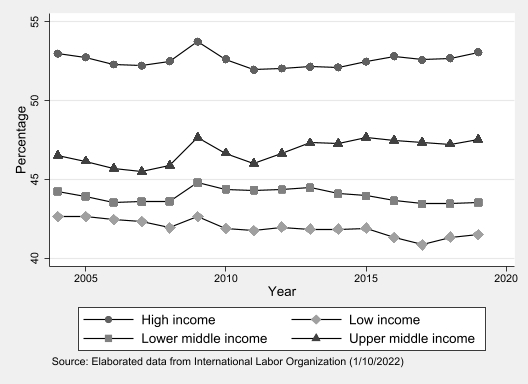
\includegraphics[width=14cm]{Income.jpg}
    \caption{Labor Share of Income for Income Group (2004-2019)}
    \label{fig:2}
\end{figure}
\begin{figure}[htp]
    \centering
    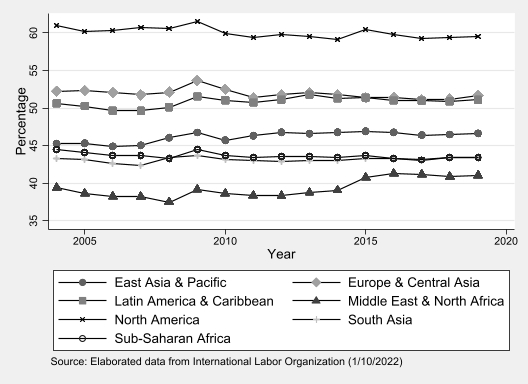
\includegraphics[width=14cm]{Region.jpg}
    \caption{Labor Share of Income by Region (2004-2019)}
    \label{fig:3}
\end{figure}
\begin{figure}[htp]
    \centering
    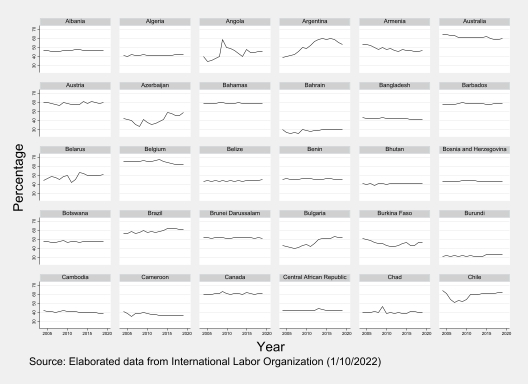
\includegraphics[width=14cm]{Countries30.jpg}
    \caption{Labor Share of Income by Country (2004-2019)}
    \label{fig:4-1}
\end{figure}
\begin{figure}[htp]
    \centering
    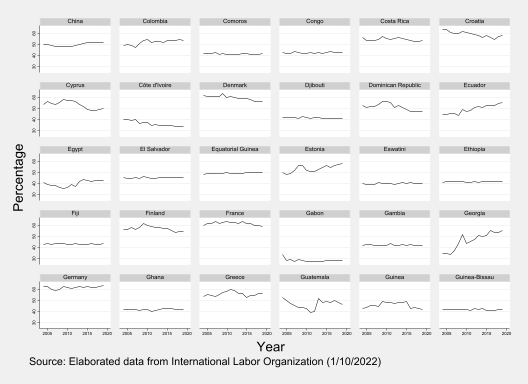
\includegraphics[width=14cm]{Countries60.jpg}
    \caption{Labor Share of Income by Country (2004-2019)}
    \label{fig:4-2}
\end{figure}
\begin{figure}[htp]
    \centering
    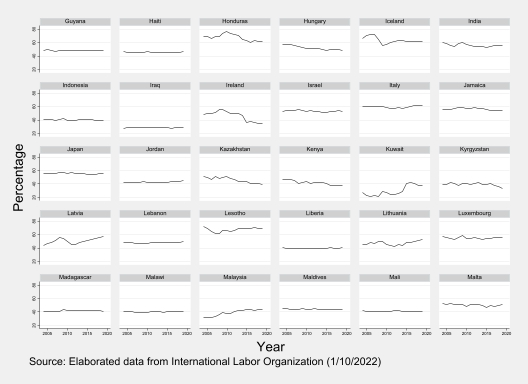
\includegraphics[width=14cm]{Countries90.jpg}
    \caption{Labor Share of Income by Country (2004-2019)}
    \label{fig:4-3}
\end{figure}
\begin{figure}[htp]
    \centering
    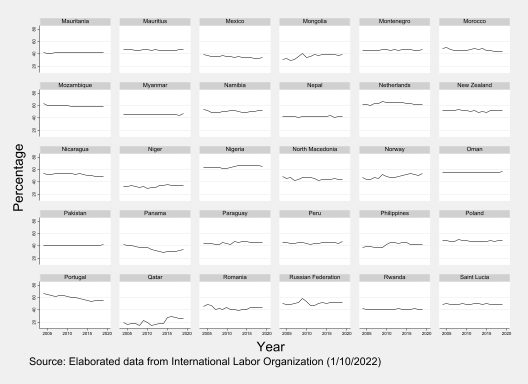
\includegraphics[width=14cm]{Countries120.jpg}
    \caption{Labor Share of Income by Country (2004-2019)}
    \label{fig:4-4}
\end{figure}
\begin{figure}[htp]
    \centering
    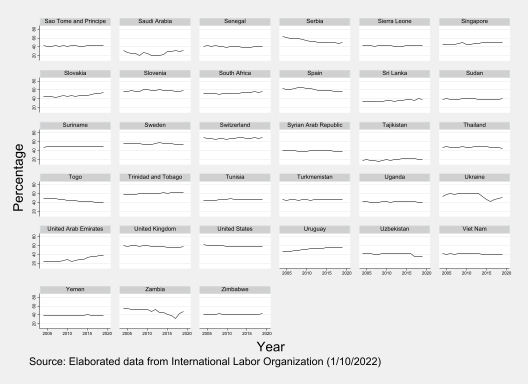
\includegraphics[width=14cm]{Countries153.jpg}
    \caption{Labor Share of Income by Country (2004-2019)}
    \label{fig:4-5}
\end{figure}

%\begin{table*}[htbp!]
%\scriptsize
%\caption{\textbf{\textit{Summary statistics - Incomegroup}}} %\label{tab:descincome}
%    \begin{center}
%       {
\def\sym#1{\ifmmode^{#1}\else\(^{#1}\)\fi}
\begin{tabular}{l*{1}{cccc}}
\hline\hline
            &        Mean&          SD&         Min&         Max\\
\hline
High income &            &            &            &            \\
lsoi        &       52.57&       10.93&       14.94&       72.46\\
rgdpna      &     1.0e+06&     2.6e+06&     3136.24&     2.1e+07\\
ctfp        &        0.83&        0.17&        0.34&        1.48\\
openess     &       -0.03&        0.20&       -0.69&        0.53\\
lcapitalint &       12.78&        0.50&       11.13&       13.80\\
\hline
Low income  &            &            &            &            \\
lsoi        &       41.92&        5.43&       29.09&       63.75\\
rgdpna      &    40748.92&    52954.82&     2134.23&     2.8e+05\\
ctfp        &        0.34&        0.13&        0.14&        0.74\\
openess     &       -0.09&        0.10&       -0.67&        0.31\\
lcapitalint &        9.41&        0.84&        8.03&       12.11\\
\hline
Lower middle income&            &            &            &            \\
lsoi        &       43.95&        8.64&       16.35&       76.48\\
rgdpna      &     3.8e+05&     1.0e+06&      436.78&     9.2e+06\\
ctfp        &        0.49&        0.21&        0.16&        1.35\\
openess     &       -0.08&        0.15&       -0.85&        0.62\\
lcapitalint &       10.73&        0.88&        8.13&       12.98\\
\hline
Upper middle income&            &            &            &            \\
lsoi        &       46.79&        6.60&       27.10&       63.96\\
rgdpna      &     7.3e+05&     2.5e+06&     1700.20&     2.1e+07\\
ctfp        &        0.62&        0.16&        0.30&        1.25\\
openess     &       -0.08&        0.18&       -0.84&        0.76\\
lcapitalint &       11.66&        0.53&       10.24&       12.86\\
\hline\hline
\end{tabular}
}

%    \end{center} 
%\centering\footnotesize Source: Own elaboration with data from ILOSTAT, World Bank and Penn World Table
%\end{table*}
%\begin{table*}[htbp!]
%\scriptsize
%\caption{\textbf{\textit{Summary statistics - Regions}}} %\label{tab:descre}
%    \begin{center}
%        {
\def\sym#1{\ifmmode^{#1}\else\(^{#1}\)\fi}
\begin{tabular}{l*{1}{cccc}}
\hline\hline
            &        Mean&          SD&         Min&         Max\\
\hline
East Asia - Pacific&            &            &            &            \\
lsoi        &       46.17&        6.93&       29.68&       64.04\\
rgdpna      &     1.8e+06&     3.9e+06&     8638.10&     2.1e+07\\
ctfp        &        0.59&        0.19&        0.24&        0.93\\
openess     &        0.00&        0.13&       -0.49&        0.41\\
lcapitalint &       11.59&        1.27&        8.13&       13.80\\
\hline
Europe - Central Asia&            &            &            &            \\
lsoi        &       51.90&        9.13&       16.35&       72.46\\
rgdpna      &     5.7e+05&     9.6e+05&     8248.29&     4.3e+06\\
ctfp        &        0.75&        0.21&        0.22&        1.45\\
openess     &       -0.08&        0.16&       -0.61&        0.76\\
lcapitalint &       12.38&        0.85&        9.63&       13.63\\
\hline
Latin America - Caribbean&            &            &            &            \\
lsoi        &       50.82&        7.85&       30.02&       76.48\\
rgdpna      &     3.2e+05&     6.7e+05&     1700.20&     3.1e+06\\
ctfp        &        0.63&        0.18&        0.34&        1.21\\
openess     &       -0.12&        0.17&       -0.84&        0.48\\
lcapitalint &       11.52&        0.62&        9.65&       12.91\\
\hline
Middle East - North Africa&            &            &            &            \\
lsoi        &       39.35&       10.17&       14.94&       56.07\\
rgdpna      &     2.9e+05&     3.5e+05&     1332.22&     1.6e+06\\
ctfp        &        0.83&        0.22&        0.51&        1.48\\
openess     &       -0.01&        0.24&       -0.85&        0.53\\
lcapitalint &       12.06&        0.91&        9.35&       13.61\\
\hline
North America&            &            &            &            \\
lsoi        &       60.02&        1.32&       58.02&       63.24\\
rgdpna      &     9.7e+06&     8.2e+06&     1.4e+06&     2.1e+07\\
ctfp        &        0.94&        0.07&        0.82&        1.00\\
openess     &       -0.02&        0.04&       -0.09&        0.06\\
lcapitalint &       12.89&        0.14&       12.55&       13.04\\
\hline
South Asia  &            &            &            &            \\
lsoi        &       43.14&        5.88&       33.03&       59.83\\
rgdpna      &     1.1e+06&     2.1e+06&     3407.32&     9.2e+06\\
ctfp        &        0.57&        0.17&        0.34&        0.80\\
openess     &       -0.09&        0.11&       -0.51&        0.06\\
lcapitalint &       10.72&        0.86&        9.30&       12.66\\
\hline
Sub-Saharan Africa&            &            &            &            \\
lsoi        &       43.65&        7.48&       27.62&       71.59\\
rgdpna      &    72656.30&     1.6e+05&      436.78&     1.0e+06\\
ctfp        &        0.47&        0.22&        0.14&        1.25\\
openess     &       -0.06&        0.16&       -0.67&        0.62\\
lcapitalint &       10.10&        1.18&        8.03&       12.86\\
\hline\hline
\end{tabular}
}

%    \end{center} 
%\centering\footnotesize Source: Own elaboration with data from ILOSTAT, World Bank and Penn World Table
%\end{table*}

\begin{table*}[htbp!]
\small
\caption{\textbf{\textit{Estimated basic regression model}}} \label{tab:firstreg}
    \begin{center}
        

{
\begin{tabular}{lccc} \hline
 & (1) & (2) & (3) \\
VARIABLES & OLS & Random Effects & Fixed Effects \\ \hline
 &  &  &  \\
openess & -13.42*** & -4.094*** & -4.029*** \\
 & (1.291) & (0.786) & (0.795) \\
dtfp & 1.855*** & 0.0213 & -0.199 \\
 & (0.434) & (0.273) & (0.276) \\
lcapitalint & 2.526*** & 0.0519 & -0.294 \\
 & (0.136) & (0.171) & (0.180) \\
Constant & 16.77*** & 46.31*** & 50.35*** \\
 & (1.449) & (2.066) & (2.065) \\
 &  &  &  \\
Observations & 2,432 & 2,432 & 2,432 \\
R-squared & 0.196 &  & 0.012 \\
 Number of id\_country &  & 152 & 152 \\ \hline
\multicolumn{4}{c}{ Robust standard errors in parentheses} \\
\multicolumn{4}{c}{ *** p$<$0.01, ** p$<$0.05, * p$<$0.1} \\
\end{tabular}
}

    \end{center} 
\end{table*}

\begin{table*}[htbp!]
\small
\caption{\textbf{\textit{Hausman test of the estimated basic regression model}}} \label{tab:haus1}
    \begin{center}
        
{
\begin{tabular}{lc} \hline
 & Values \\ \hline
 &  \\
Chi-Squared Statistic & 58.84 \\
P value & 0.0000 \\ \hline
\multicolumn{2}{c}{Test of H0: Difference in coefficients not systematic} \\
\multicolumn{2}{c}{Source: Own elaboration} \\
\end{tabular}
}

    \end{center} 
\end{table*}

\begin{table*}[htbp!]
\small
\caption{\textbf{\textit{Estimated basic regression model with crisis}}} \label{tab:second reg}
    \begin{center}
        {
\begin{tabular}{lccc} \hline
 & (1) & (2) & (3) \\
VARIABLES & OLS & Random Effects & Fixed Effects \\ \hline
 &  &  &  \\
openess & -13.44*** & -4.140*** & -4.075*** \\
 & (1.289) & (0.783) & (0.792) \\
dtfp & 1.842*** & -0.0177 & -0.235 \\
 & (0.434) & (0.272) & (0.274) \\
lcapitalint & 2.531*** & 0.0807 & -0.260 \\
 & (0.136) & (0.171) & (0.180) \\
crisis & 1.163 & 1.028*** & 1.015*** \\
 & (0.736) & (0.216) & (0.214) \\
Constant & 16.64*** & 45.93*** & 49.91*** \\
 & (1.452) & (2.060) & (2.057) \\
 &  &  &  \\
Observations & 2,432 & 2,432 & 2,432 \\
R-squared & 0.197 &  & 0.022 \\
 Number of id\_country &  & 152 & 152 \\ \hline
\multicolumn{4}{c}{ Robust standard errors in parentheses} \\
\multicolumn{4}{c}{ *** p$<$0.01, ** p$<$0.05, * p$<$0.1} \\
\end{tabular}
}

    \end{center} 
\end{table*}

\begin{table*}[htbp!]
\small
\caption{\textbf{\textit{Hausman test of the estimated basic regression model with crisis}}} \label{tab:haus1}
    \begin{center}
        
{
\begin{tabular}{lc} \hline
 & Values \\ \hline
 &  \\
Chi-Squared Statistic & 57.78 \\
P value & 0.0000 \\ \hline
\multicolumn{2}{c}{Test of H0: Difference in coefficients not systematic} \\
\multicolumn{2}{c}{Source: Own elaboration} \\
\end{tabular}
}

    \end{center} 
\end{table*}


\begin{table*}[htbp!]
\small
\caption{\textbf{\textit{Estimated basic regression model with crisis and income groups}}} \label{tab:third reg}
    \begin{center}
        
\begin{tabular}{lccc} \hline
 & (1) & (2) & (3) \\
VARIABLES & OLS & Random Effects & Fixed Effects \\ \hline
 &  &  &  \\
openess & -13.68*** & -4.214*** & -4.075*** \\
 & (1.290) & (0.781) & (0.792) \\
dtfp & 0.738* & -0.0990 & -0.235 \\
 & (0.433) & (0.273) & (0.274) \\
lcapitalint & 2.406*** & 0.0158 & -0.260 \\
 & (0.132) & (0.171) & (0.180) \\
incg & -1.176*** & -2.056*** & ommited \\
 & (0.142) & (0.562) &  \\
crisis & 1.184 & 1.026*** & 1.015*** \\
 & (0.728) & (0.215) & (0.214) \\
Constant & 21.36*** & 51.78*** & 49.91*** \\
 & (1.429) & (2.612) & (2.057) \\
 &  &  &  \\
Observations & 2,432 & 2,432 & 2,432 \\
R-squared & 0.214 &  & 0.022 \\
 Number of id\_country &  & 152 & 152 \\ \hline
\multicolumn{4}{c}{ Robust standard errors in parentheses} \\
\multicolumn{4}{c}{ *** p$<$0.01, ** p$<$0.05, * p$<$0.1} \\
\end{tabular}


    \end{center} 
\end{table*}

\begin{table*}[htbp!]
\small
\caption{\textbf{\textit{Hausman test of the estimated basic regression model with crisis and income groups}}} \label{tab:haus1}
    \begin{center}
        
{
\begin{tabular}{lc} \hline
 & Values \\ \hline
 &  \\
Chi-Squared Statistic & 42.46 \\
P value & 0.0000 \\ \hline
\multicolumn{2}{c}{Test of H0: Difference in coefficients not systematic} \\
\multicolumn{2}{c}{Source: Own elaboration} \\
\end{tabular}
}

    \end{center} 
\end{table*}

\clearpage
\section{Do-file}\label{Do-file}
\lstset{
  basicstyle=\ttfamily,
  columns=fullflexible,
  frame=single,
  breaklines=true
}
 \lstinputlisting{lso.do}
 

\end{document}